% Bachelor Thesis Webperformance für den mobilen Endanwender
% von Andreas Lorer
% 2015
% Studiengang: Angewandte Informatik - HS Ravensburg-Weingarten
\documentclass[a4paper,11pt,singlespacing]{article}
\usepackage[left=2.5cm,right=2.5cm,top=2.5cm]{geometry}
\usepackage[hyphens]{url}
\usepackage[backend=biber,style=alphabetic,backref=true,citecounter=true,citestyle=authoryear]{biblatex}
\usepackage{csquotes}
\usepackage{hyperref}
\usepackage{setspace}
\usepackage[utf8]{inputenc}
\usepackage[T1]{fontenc}
\usepackage[ngerman]{babel}
\usepackage{color}
\usepackage{hyperref}
\usepackage{pdflscape}
\usepackage{graphicx}
\usepackage{listings}
\usepackage{csquotes}
\addbibresource{sections/zitate.bib}
\pagestyle{myheadings}
\markright{\centerline{Webperformance für den mobilen Endanwender}}
\author{Andreas Lorer}

\graphicspath{{images/}}            
\setlength{\parindent}{0ex}  	% Absatzeinrueckung verhindern

\definecolor{mygreen}{rgb}{0,0.6,0}
\definecolor{mygray}{rgb}{0.5,0.5,0.5}
\definecolor{mymauve}{rgb}{0.58,0,0.82}

\newenvironment{italicquotes}
{\begin{quote}\itshape}
{\end{quote}}

\begin{document}
  % document styles for listings
  \lstset{
    backgroundcolor=\color{white},
    basicstyle=\footnotesize\ttfamily,
    breakatwhitespace=true,
    breaklines=true,
    numbers=left,
    numbersep=5pt,
    deletekeywords={event}, 
    numberstyle=\tiny,
    showspaces=false,
    showtabs=false,
    language=html,
    keywordstyle=\bfseries\color{mymauve},
    commentstyle=\itshape\color{mygreen},
    columns=fullflexible,
    xleftmargin=0.5cm,
    xrightmargin=1cm,
    frame=lr,
    framesep=8pt,
    framerule=0pt
  }

	%Deckblatt
	\newcommand{\headline}{Bachelor-Thesis}
	\newcommand{\subheadline}{Webperformance für den mobilen Endanwender}
	\begin{titlepage}
  \begin{center}

    % Upper part of the page
    
\includegraphics[width=0.5\textwidth]{../deckblatt/images/logo.png}\\[2cm]    
    {\huge \bfseries \headline}\\[0.5cm]
    {\huge \bfseries \subheadline}\\[0.5cm]
    {\huge \bfseries \subsubheadline}\\[0.5cm]
    
   % Zusammenfassung
    \begin{abstract}
      \noindent
       \\[1cm]
    \end{abstract}

    {\large \today}\\[1cm]
    \vspace{2cm}

	\begin{flushleft}
      \hspace*{3cm} Columbus Interactive\\
      \hspace*{3cm} Eywiesenstraße 6\\
      \hspace*{3cm} 88212 Ravensburg\\
      \vspace{1cm}
      \hspace*{3cm} Fakultät Elektrotechnik und Informatik\\
      \hspace*{3cm} Studiengang Angewandte Informatik\\
      \hspace*{3cm} Hochschule Ravensburg-Weingarten\\
      \hspace*{3cm} Doggenriedstraße, 88250 Weingarten

    \end{flushleft}

    \vspace{1.5cm}

    % Authoren
    \begin{flushleft}\large
	  \hspace*{2cm} \emph{Autor:}\\
	  \hspace*{2cm} Andreas Lorer\\
	  \hspace*{2cm} \href{mailto:andreas.lorer@hs-weingarten.de}{\nolinkurl{andreas.lorer@hs-weingarten.de} }\\
      \hspace*{2cm} 88250 Weingarten\\
      \hspace*{2cm} Wilhelmstraße 4
    \end{flushleft}
   \end{center}
   \vfill
\end{titlepage}

	
	%Inhaltsverzeichnis
	\tableofcontents 
	\thispagestyle{empty}
	\pagebreak

	\setcounter{page}{1}

\section{Einleitung} % (fold)
\label{sec:einleitung}
	Diese Arbeit beschäftigt sich umfassend mit dem Thema Web Performance unter dem Aspekt, dass immer mehr Anwender mittels Smartphone mit dem Web agieren. Sie soll die Frage klären, warum Webanwendungen auf einem Smartphone oftmals um ein Vielfaches langsamer Laden, als via Desktop-PC, welche Auswirkungen sich daraus ergeben und welche Maßnahmen zur Optimierung ergriffen werden können. Daraus resultiert ein \texttt{Workflow}, der sich nach den "`Best Practices"' richtet. Die Arbeit endet mit den kulturellen Veränderungen, die das Thema Web Performance für ein Unternehmen mit sich bringen kann und welche Herausforderungen es zu meistern gilt.

	\subsection{Motivation} % (fold)
	\label{sub:motivation}

		Niemand mag es, zu warten. Sei es auf Bus, Bahn oder an der Kasse im Supermarkt. Wir warten auch nicht gerne im Internet auf das Buffern eines Videos, beim Besuch einer Webseite oder beim Shoppen via App. Zu oft wird aus dem "`nur mal eben diesen Begriff nachschlagen"' ein endloses Starren auf den weißen Bildschirm. Jeder kennt das.\\

		Larry Page, CEO und Mitgründer von Google, sagt:
		\begin{quote}
			\textit{"`As a product manager you should know that speed is the number one feature."'}\autocite{holzle10}
		\end{quote}
		Niemand mag es, zu warten, auch nicht auf eine Webanwendung. Die Studie "`The Psychology of Web Performance"' zitierte bereits im Jahr 2008 folgende Ergebnisse:

		\begin{quote}\itshape
			"`Slow web pages lower perceived credibility and quality. Keep your page load times below tolerable attention thresholds, and users will experience less frustration, lower blood pressure, deeper flow states, higher conversion rates, and lower bailout rates. Faster websites are actually perceived to be more interesting and attractive."' \autocite{webOpti08}
		\end{quote}

		Das Hauptvermarktungsargument für den Chrome Browser war damals, er sei schneller als die Konkurrenz. Tatsächlich ist für Google Geschwindigkeit alles. Deshalb hat Google im Jahr 2010 angekündigt, dass Geschwindigkeit in die Berechnung des \texttt{Google Page Rankings} mit einfließt.

		\begin{quote}\itshape
			"`Faster sites create happy users and we've seen in our internal studies that when a site responds slowly, visitors spend less time there. [...] Recent data shows that improving site speed also reduces operating costs. Like us, our users place a lot of value in speed — that's why we've decided to take site speed into account in our search rankings"'\autocite{google10}
		\end{quote}

		Aktuell (2015) geht Google sogar noch einen Schritt weiter und informiert tausende Webmaster per E-Mail über die schlechte Usability ihrer Websites für mobile Besucher und warnt ausdrücklich vor dementsprechend "`angepassten Rankings"'.\autocite{t3n15}
		Im Hinblick auf die Zukunft wird der Marktanteil an mobilen Internetnutzern noch weiter wachsen und die Optimierung der Ladezeiten gewinnt dadurch noch mehr an Bedeutung. Zwischen 2011 und 2014 stieg die Anzahl der Smartphonenutzer von 18\% auf 50\% an. Dies ist ein Wachstum von 32\% innerhalb von nur 3 Jahren.\autocite{tns14}\\

		\begin{figure}[htbp]
			\begin{center}
				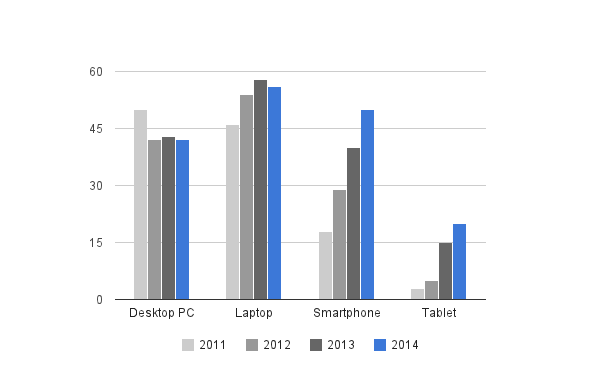
\includegraphics[width=0.75\textwidth]{smartphoneUsage.png}
			\end{center}
			\caption{Gerätenutzung in der Gesamtbevölkerung (2011 – 2014)\autocite{tns14}}
			\label{fig:geraetenutzung}
		\end{figure}

		Die Antwort auf diesen Trend läutete eine Ära ein, die wir heute unter dem Namen \texttt{Responsive Webdesign} kennen. "`Responsive"' muss aber sehr viel mehr bedeuten, als nur eine angepasste Darstellung für eine bestimmte Art von Gerät. \textit{"`Two out of three mobile shoppers expect pages to load in 4 seconds or less."'} \autocite{radware13}. Der Anwender erwartet also auf dem Smartphone ähnliche oder gleiche Ladezeiten wie er sie auch von der Nutzung des Desktop Pc's gewohnt ist. Diese Erwartungen werden von dem Großteil der Internetseiten nicht erfüllt. Der Inhalt einer Seite muss darum so aufbereitet werden, dass dieser auch auf Geräten mit langsamer Internetverbindung, hoher Latenz und einem begrenzten Datentarif, in einer für den Anwender annehmbaren Geschwindigkeit, angezeigt werden kann.\\

	% subsection motivation (end)



	\subsection{Zielsetzung} % (fold)
	\label{sub:zielsetzung}
		Um gängige Methoden und Techniken der Ladezeit-Optimierung anzuwenden, wird das Projekt anhand der Website \url{http://andreaslorer.de/old/} durchgeführt. Das Ziel ist es, die Ladezeit der Website auf dem Smartphone, wie auch auf dem Desktop auf unter 1000 Millisekunden zu verringern. Mit Ladezeit ist dabei nicht die Zeit gemeint, die benötigt wird, um die Website komplett zu laden, sondern die Zeit, bis eine erste visuelle Rückmeldung für den Anwender zu sehen ist. Diese, vom Anwender wahrgenommene Rückmeldung, nennt man auch "`Perceived Performance"' und bedeutet, dass die Ladezeit als schneller empfunden wird, als es eigentlich laut Messwerten der Fall ist. Näheres dazu wird in Punkt \ref{sub:perceived_performance} beschrieben.\\

	% subsection zielsetzung (end)



	\subsection{Eigene Leistung} % (fold)
	\label{sub:eigene_leistung}
		Die Leistung besteht darin, einen Gesamtüberblick über die heutigen Best Practices zu ermöglicht. Die Arbeit soll dem Leser ein Gespühr für Fehler in der Struktur von Webanwendungen geben, die für die Geschwindigkeit hinderlich sind.
		Es soll herausgefunden werden, was getan werden muss um die Ladezeit zu minimieren, wie ein moderner "`Workflow"' aussehen kann, damit eine Webanwendung schon bei seiner Entstehung schnell lädt und im Projektverlauf schnell bleibt. Des Weiteren soll erklärt werden, welche Herausforderungen es zu meistern gilt um eine schnelle Webanwendung zu erreichen, welche Tools es gibt und welche Vor- oder Nachteile diese mit sich bringen.\\
		Diese Arbeit befasst sich nicht mit der Geschwindigkeit von Datenbanken, SQL-Abfragen oder sonstigen Problemen, die durch einen Engpass ein schnelles Laden der Seite verhindern könnten.

	% subsection eigene_leistung (end)



	\subsection{Ist-Zustand} % (fold)
	\label{sub:ist_zustand}
		Die Webseite \url{www.andreaslorer.de}  ist auf einem \texttt{Shared Hosting}
		\footnote{Bei shared Hosting werden mehrere Websites von verschiedenen Website-Betreibern von dem gleichen Webserver gehostet. Bei Shared Hosting teilen sich in der Regel Hunderte andere Websites einen Server \autocite{itWissen}} 
		aufgesetzt und die Antwortzeit des Servers beträgt circa <200 Millisekunden. Dadurch, dass es keine Möglichkeit gibt, \texttt{Root Rechte}\footnote{Standardmäßig existiert unter Linux immer ein Konto für den Benutzer "`root"' mit der User-ID 0. Dies ist ein Systemaccount mit vollem Zugriff auf das gesamte System, und damit auch auf alle Dateien und Einstellungen aller Benutzer \autocite{ubuntu14}} auf einem Shared Hosting zu bekommen, können so manche serverseitige Einstellungen nicht durchgeführt werden. Diese werden dann zwar aufgezeigt, kommen aber für dieses Projekt nicht zum Einsatz.\\
		Die Website hat als Ausgangsbasis einen einfachen Aufbau. Sie besteht aus einer Bilder Gallerie basierend auf PHP und dem Bootstrap Framework.
	% subsection ist_zustand (end)



\pagebreak
%
% section einleitung (end)
%

	\pagebreak

	\printbibliography

 % 	\bibliographystyle{apalike}
 % 	\bibliography{sections/zitate}
	\end{document}